%%%% main.tex -- Canvas3D: A Unified 3D-Aware Framework for Painting Animation
%%%% via Object-Level Decomposition, Monocular 3D Lifting, Line-Art Composition,
%%%% and Geometry-Grounded Video Synthesis
%%%% IJCAI 2027 submission
%%%% Based on the official IJCAI--ECAI 26 template (ijcai26.sty).

\typeout{IJCAI 2027 Submission: Canvas3D}

\documentclass{article}
\pdfpagewidth=8.5in
\pdfpageheight=11in

\usepackage{ijcai26}

% Use the postscript times font!
\usepackage{times}
\usepackage{soul}
\usepackage{url}
\usepackage[hidelinks]{hyperref}
\usepackage[utf8]{inputenc}
\usepackage{xeCJK}   % CJK support (compile with XeLaTeX)
\setCJKmainfont{SimSun}[AutoFakeBold=true,AutoFakeSlant=true]
\usepackage[small]{caption}
\usepackage{graphicx}
\usepackage{amsmath}
\usepackage{amsthm}
\usepackage{amssymb}    % for \mathbb{R}, \mathbb{E}
\usepackage{natbib}   % required for \citet / \citep
\usepackage{booktabs}
\usepackage{algorithm}
\usepackage{algorithmic}
\usepackage{multirow}
\usepackage{pifont}       % for \ding{55} (cross) and \ding{51} (check)
\usepackage[switch]{lineno}
\usepackage{microtype}    % improve paragraph breaking, reduce overfull boxes

% TikZ for high-quality architecture diagrams
\usepackage{tikz}
\usetikzlibrary{
    shapes, arrows, arrows.meta, positioning, fit,
    backgrounds, calc, decorations.pathreplacing,
    decorations.pathmorphing, shadows, shapes.geometric,
    shapes.multipart, patterns, matrix, chains,
    decorations.markings, decorations.text
}

% Custom TikZ styles
\tikzset{
    modbox/.style={
        draw=black!60, fill=blue!5, rounded corners=3pt,
        minimum width=2.8cm, minimum height=1.0cm,
        align=center, font=\footnotesize,
        thick
    },
    modbox_blue/.style={
        modbox, fill=blue!5
    },
    modbox_green/.style={
        modbox, fill=green!5
    },
    modbox_orange/.style={
        modbox, fill=orange!5
    },
    modbox_purple/.style={
        modbox, fill=purple!5
    },
    modbox_red/.style={
        modbox, fill=red!5
    },
    dataarrow/.style={
        ->, >=Stealth, thick, draw=black!50
    },
    dataarrow_blue/.style={
        ->, >=Stealth, thick, draw=blue!60
    },
    dataarrow_red/.style={
        ->, >=Stealth, thick, draw=red!60
    }
}

% Comment out this line in the camera-ready submission
\linenumbers

\urlstyle{same}

\newtheorem{example}{Example}
\newtheorem{theorem}{Theorem}
\newtheorem{definition}{Definition}

% \pdfinfo is pdftex-only; guard it so XeLaTeX can compile this file too.
\ifdefined\pdfinfo
\pdfinfo{
/TemplateVersion (IJCAI.2026.0)
}
\fi

% =====================================================================
%  Title and authors
% =====================================================================
\title{Canvas3D: Object-Level 3D Lifting and Line-Art Composition\\
for Painting Animation}

\author{
    Anonymous Authors
    \affiliations
    AIforEducation Project
    \emails
    aiforeducation@example.com
}

\begin{document}

\maketitle

% =====================================================================
%  Abstract  (rewritten for IJCAI 2027: idea-centric, no model names)
% =====================================================================
\begin{abstract}
Animating static artworks---oil paintings, ink-wash scrolls, and
frescoes---into explorable, narratively coherent videos is a long-standing
goal at the intersection of computer vision, generative modeling, and digital
cultural heritage. Existing approaches remain bifurcated: image-to-video
diffusion models produce visually fluent motion but collapse three-dimensional
structure under viewpoint change, while feed-forward 3D reconstruction
pipelines capture geometry at the cost of obliterating painterly texture,
impasto, and brushstroke identity. The root cause is a fundamental
\emph{objective tension}: artistic style fidelity and 3D scene structure are
governed by incompatible optimization targets, and no single end-to-end model
satisfies both, especially when the task demands object-level manipulation.
We propose \textbf{Canvas3D}, a framework that resolves this tension through
a \emph{modular decomposition of concerns}. Rather than training a monolithic
network, Canvas3D factors the painting-to-video problem into four
independently optimized, mutually reinforcing sub-problems:
\emph{(i) perceptual grouping} of a painting into semantically meaningful
foreground objects and a preserved background, jointly with monocular
depth-derived layer ordering; \emph{(ii) per-object geometric lifting} that
converts each 2D region into a metric-scaled 3D representation and assembles
a reusable, retrievable object-level model library; \emph{(iii) line-art
scene composition} in which hand-drawn sketches serve as \emph{spatial
constraints} rather than stylistic hints, solved by a contour-based rigid
registration that places each 3D object at its sketched location and a
depth-conditioned inpainting module that restores disoccluded background
texture in a geometry-aware manner; and \emph{(iv) geometry-grounded video
synthesis} that renders the composited 3D scene into multi-view keyframes
and injects depth and edge cues as dual control signals into a video
diffusion backbone, anchoring temporal motion to explicit 3D structure
rather than learned heuristics. The key insight is that \emph{separating
perceptual, geometric, compositional, and temporal concerns} turns an
ill-posed, conflicting joint problem into four well-posed sub-problems,
each addressable by an off-the-shelf specialist, while their interaction
yields capabilities---arbitrary object repositioning, multi-view
explorability, and style-anchored animation---that no single-modality
pipeline offers. On a curated benchmark of classical paintings, Canvas3D
achieves state-of-the-art style fidelity, perceptual quality, and temporal
coherence, with user studies confirming strong preference for artistic
authenticity, motion naturalness, and compositional-intent alignment.
\end{abstract}

% =====================================================================
%  Body: each section lives in its own file under sec/
% =====================================================================
% =====================================================================
%  Section: Introduction  (IJCAI 2027 revision: idea-centric)
% =====================================================================
\section{Introduction}
\label{sec:intro}

Classical paintings---whether oil on canvas, ink on silk, or pigment on
fresco---are cultural artifacts that encode centuries of human visual
imagination~\cite{lowenthal2015heritage}. From van Gogh's swirling
\textit{Starry Night} to Zhang Zeduan's panoramic \textit{Along the River
During the Qingming Festival}, these works imply motion, narrative, and
spatial depth that their static medium can only suggest. Animating such
paintings as explorable videos has therefore emerged as a compelling
research goal at the intersection of computer vision, generative
modeling, and digital cultural
heritage~\cite{zhang2024artgallery,dong2024enhancingpainting}.

Recent years have witnessed remarkable progress on two fronts that,
however, fail to meet on common ground. On one hand, image-to-video
(I2V) diffusion models~\cite{blattmann2023svd,wan2025,ltxvideo2024,
yang2025cogvideox}, combined with controllable conditioning
mechanisms~\cite{zhang2023controlnet,wang2024easycontrol,peng2024controlnext},
can animate a single photograph into a short clip with plausible
per-frame dynamics. Yet when applied directly to oil paintings or
ink-wash artworks, they suffer from two fundamental shortcomings.
First, they operate entirely in 2D pixel space: the model has no
geometric understanding of object depth ordering, self-occlusion, or
relative spatial layout, and consequently cannot synthesize novel
viewpoints or maintain consistent 3D structure across frames. Second,
long-range temporal coherence degrades rapidly beyond 2--4 seconds, as
the latent-space interpolation lacks explicit geometric constraints to
anchor the motion trajectory.

On the other hand, 3D reconstruction and rendering
methods~\cite{mildenhall2020nerf,kerbl20233dgs,huang20242dgs} can
reconstruct explorable 3D scenes from sparse views, and feed-forward
monocular variants~\cite{wang2024triposplat,tang2024dreamgaussian,
charatan2024pixelsplat} can even lift a single image to a 3D
representation. However, these reconstruction pipelines are optimized
for photorealistic fidelity; when applied to paintings, the rendering
process replaces expressive brushstrokes with geometric artifacts,
flattens the impasto texture, and bleeds semantic color boundaries
under novel-view projection.

The core tension is this: \emph{3D scene structure and artistic style
fidelity} are governed by incompatible optimization objectives, and no
single model family---neither pure diffusion nor pure 3D
reconstruction---satisfactorily achieves both. This tension becomes
especially acute when the animation task requires
\textbf{object-level manipulation}: moving a painted figure from one
compositional position to another while preserving its painterly
identity and filling the resulting gaps with plausible background
content.

\smallskip
\noindent\textbf{Our approach: modular separation of concerns.}
Rather than training a single monolithic network to jointly optimize
style and structure---an ill-posed objective whose gradients pull in
opposite directions---we propose to \emph{factor} the painting-to-video
problem into four interacting yet independently optimized sub-problems,
each addressed by a specialist and communicating with the next through
a small, interpretable handshake representation
(Figure~\ref{fig:overview}):

\begin{itemize}
    \item \textbf{PaintParse} handles \emph{perceptual grouping}:
    decomposing the input painting into foreground objects and a
    background layer using an art-domain-adapted segmentation backbone,
    augmented with monocular depth estimation for metric-scale layer
    ordering.
    \item \textbf{MonoSplat} handles \emph{geometric structure}:
    lifting each segmented foreground region into a high-fidelity 3D
    representation via feed-forward single-image 3D prediction,
    assembling an object-level model library with depth-derived metric
    rescaling.
    \item \textbf{SketchComp} handles \emph{compositional intent}:
    accepting hand-drawn line-art sketches specifying target object
    positions, solving a contour-based rigid registration to place each
    3D object onto its sketch, and filling disocclusion gaps through a
    depth-conditioned inpainting module that preserves background
    artistic texture.
    \item \textbf{ArtiFlow} handles \emph{temporal rendering}: rendering
    the composited 3D scene into multi-view keyframes and feeding them
    into a video diffusion backbone with dual control branches
    (depth + edge), producing temporally smooth animations with
    pixel-precise object motion governed by explicit 3D geometry
    rather than learned heuristics.
\end{itemize}

This decomposition enables a clean separation of concerns, and the
handshakes carry exactly the information each downstream stage needs
and no more, preventing error compounding. The result is a system that
supports \emph{arbitrary object repositioning}, \emph{multi-view
explorability}, and \emph{style-anchored animation}---capabilities
that no prior single-modality pipeline offers.

\smallskip
\noindent\textbf{Contributions.} Our contributions are:
\begin{enumerate}
    \item \textbf{A modular factorization} of the painting-to-video
    problem into four independently optimized specialists---PaintParse
    (perceptual grouping), MonoSplat (per-object 3D lifting),
    SketchComp (line-art composition with depth-aware inpainting), and
    ArtiFlow (dual-conditioned video synthesis)---communicating through
    interpretable handshake representations. To our knowledge this is
    the first end-to-end pipeline for 3D-aware, artistically
    controllable painting animation.
    \item \textbf{An object-level 3D lifting pipeline} (MonoSplat) that
    combines art-domain-adapted instance segmentation with feed-forward
    monocular 3D prediction and depth-derived metric rescaling,
    producing a reusable, retrievable library of 3D foreground objects
    from a single painting.
    \item \textbf{A sketch-conditioned 3D scene composition algorithm}
    (SketchComp) with a contour-based rigid registration that jointly
    optimizes region IoU and boundary Chamfer distance, and a
    depth-aware color inpainting module that fills disocclusion gaps
    while preserving the background's artistic texture.
    \item \textbf{A geometry-grounded video synthesis workflow}
    (ArtiFlow) with dual control branches (depth + edge) and
    first-frame latent anchoring for explicit 3D-structure-anchored
    animation with per-object motion control.
    \item \textbf{Comprehensive evaluation} on a curated benchmark of
    50 classical oil paintings and ink-wash works, achieving
    state-of-the-art style fidelity, perceptual quality, and temporal
    coherence, with user studies confirming strong preference for
    artistic authenticity, motion naturalness, and compositional-intent
    alignment.
\end{enumerate}

% =====================================================================
%  Section: Related Work  (IJCAI 2027 revision: distilled lineage)
% =====================================================================
\section{Related Work}
\label{sec:related}

We organize prior work along the four axes that motivate our modular
decomposition, tracing the developmental lineage of each thread and
positioning Canvas3D at their intersection.

\subsection{From Pixel-Level Stylization to Painting Animation}

The earliest approaches to painting animation treat the input as a
\emph{pixel grid to be stylized over time}. Static image style transfer,
pioneered by feature-correlation methods~\cite{gatys2016image} and extended
by fast feed-forward networks~\cite{johnson2016perceptual,huang2017arbitrary}
and transformer-based stylizers~\cite{deng2021stytr2}, established that
artistic appearance can be re-injected into arbitrary content. Video style
transfer then addressed temporal coherence through optical-flow
regularization~\cite{ruder2016artistic,chen2017coherent,wang2020consistent},
multi-channel correlation~\cite{deng2021arbitrary}, and content deformation
fields~\cite{ouyang2024codef}. A second lineage pursues
\emph{stroke-level synthesis}---reproducing the physical painting process as
a time-lapse~\cite{zhao2020painting,zou2021stylized,liu2021neuralstrokes}---but
such methods reconstruct \emph{how a painting was made} rather than
\emph{how its subjects could move}. A third, narrower thread drives
\emph{portrait motion} on painted faces~\cite{guo2024liveportrait,tan2024edtalk}
but cannot animate full-body figures or background elements. The diffusion
era introduced inversion-based stylization~\cite{zhang2023inversion} and
video-consistent editing~\cite{ceylan2023pix2video,chai2023stablevideo,geyer2023tokenflow,liang2024flowvid},
which preserve appearance under text-driven edits but provide no geometric
handle on object pose. The recent InkSpirit~\cite{zhang2025inkspirit} and
StyleMaster~\cite{ye2025stylemaster} push appearance fidelity further yet
remain confined to 2D image translation. Across this lineage, the persistent
gap is the absence of \emph{object-level, 3D-grounded motion control}:
appearance is preserved, but spatial structure is not.

\subsection{3D Scene Representations and Single-Image Lifting}

Three-dimensional representations evolved from implicit radiance
fields~\cite{mildenhall2020nerf} to explicit primitives. 3D Gaussian
Splatting~\cite{kerbl20233dgs} represents a scene as a set of anisotropic
Gaussians with differentiable rasterization, enabling real-time
photorealistic rendering; 2D Gaussian Splatting~\cite{huang20242dgs}
collapses the third scale dimension into a surface normal, improving
geometric fidelity for surface-like content. Crucially, the field has
recently shifted from \emph{per-scene optimization} to \emph{feed-forward
single-image lifting}: generative-prior methods~\cite{tang2024dreamgaussian}
predict 3D assets from one image, while state-of-the-art feed-forward
predictors~\cite{wang2024triposplat,charatan2024pixelsplat,jiang2025anysplat}
regress Gaussian parameters directly, with two-view and unconstrained-view
variants broadening the input regime. These advances make it feasible to
lift individual painting regions into 3D, but none addresses the downstream
challenge of \emph{composing multiple such objects into a coherent,
artistically controllable scene}---exactly the gap our framework targets.

\subsection{Sketch and Line-Art as a Composition Interface}

Hand-drawn sketches have a long history as an intuitive interface for shape
prototyping~\cite{olson2011sketch}. Recent work demonstrates that
contour-level spatial reasoning is tractable with modern vision models:
ShadowDraw~\cite{luo2026shadowdraw} generates compositional shadow art from
object inputs, LineArt~\cite{wang2024lineart} performs training-free
appearance transfer onto design drawings via diffusion, and region-aware
simplification~\cite{nguyen2024region} and volumetric animation
toolkits~\cite{foxgieg2024lightning} illustrate the expressive potential of
hand-drawn control. In diffusion-based generation, sketches typically serve
as a \emph{stylistic} or \emph{boundary} condition (e.g., ControlNet-style
edge injection~\cite{zhang2023controlnet}). Canvas3D departs from this
convention by treating line-art as a \emph{spatial constraint} that
resolves the which-object-where problem in 3D scene assembly: a sketch is
not merely an appearance hint but a target silhouette that a 3D object is
geometrically registered to.

\subsection{Controllable Image-to-Video Generation}

The leap from text-to-image to text-to-video was powered by diffusion
transformers~\cite{peebles2023dit} and video diffusion
models~\cite{ho2022vdm,ho2022video}. A family of scalable
backbones~\cite{yang2025cogvideox,wan2025,ltxvideo2024,blattmann2023svd}
now supports high-fidelity image-to-video synthesis. Controllability has
been pursued through auxiliary conditioning:
ControlNet~\cite{zhang2023controlnet} injects edge, depth, and pose maps
into the diffusion U-Net, with video extensions~\cite{wang2024easycontrol}
and efficiency-oriented variants~\cite{peng2024controlnext} broadening its
applicability. Cinematic shot design~\cite{xing2025motioncanvas} and
clipart animation~\cite{wu2025aniclipart} demonstrate compelling 3D-aware
control without explicit 3D supervision. Despite these advances, existing
I2V control methods are confined to \emph{per-frame conditioning
signals}: they cannot reason about 3D object identity, depth ordering, or
occlusion across frames, and consequently drift under viewpoint change.
Canvas3D addresses this by grounding all control signals in an explicit,
object-level 3D scene that is composited, rendered, and then fed into the
video diffusion backbone.

\subsection{Painting-Specific Animation Pipelines}

A small but growing body of work targets paintings directly. Domain-adapted
detectors~\cite{chen2025pldsyolo} and art-segmentation
datasets~\cite{saleh2016metric} establish that natural-image segmentation
backbones~\cite{jocher2023yolov8,wang2024yolov9,wang2024yolov10,tian2025yolov12}
and foundation segmentation models~\cite{kirillov2023sam,ravi2024sam2}
require art-specific fine-tuning due to brushstroke texture and intentional
boundary blending. Chinese ink-wash style transfer has been explored via
instance-aware coherence~\cite{liang2021instance} and staged diffusion
guidance~\cite{liu2026chipdiff}. Most relevant to our setting,
``Printing the Underdetermined''~\cite{ming2026printing} translates
paintings to 3D representations via video generative models but operates
on the entire image jointly rather than at the object level, while
OilPaintingRevive~\cite{oilpaintingrevive2026} proposes a multi-stage
pipeline combining 2DGS with video refinement, but its skeleton-binding
network requires per-scene optimization that limits compositional
flexibility. Canvas3D advances beyond these works along four
axes---\emph{object-level} rather than image-level manipulation,
\emph{line-art} as a compositional control interface,
\emph{depth-aware inpainting} for disocclusion, and
\emph{multi-modal geometric conditioning} for video synthesis---yielding
stronger 3D consistency and explicit compositional control.

% =====================================================================
%  Section: Method  (IJCAI 2027 revision: design-rationale centric)
% =====================================================================
\section{Method}
\label{sec:method}

\paragraph{Design philosophy.}
A single painting-animation system must simultaneously satisfy four
\emph{conflicting} objectives: perceptual grouping of artistically rendered
content, geometric reconstruction of objects that have no real 3D extent,
user-specifiable composition, and temporally coherent stylized rendering.
Jointly optimizing a single network for all four is ill-posed because the
gradients of style fidelity and 3D structure pull in opposite directions.
Our central design principle is therefore \emph{modular separation of
concerns with explicit handshakes}: each objective is addressed by an
independently optimized specialist, and the four specialists communicate
only through well-defined, interpretable intermediate
representations---masks with depth-ordered layers, a metric-scaled
object-level 3D library, a composited 3D scene with disocclusion-filled
background, and finally a multi-view keyframe stream with paired
geometry and edge cues. This decomposition converts a conflicting joint
problem into four well-posed sub-problems, while the handshakes carry
exactly the information each downstream stage needs and no more,
preventing error compounding.

\paragraph{Problem statement.}
Given a painting scan $P \in \mathbb{R}^{H\times W \times 3}$ and a set of
hand-drawn line-art sketches $L = \{\ell_1, \dots, \ell_K\}$ specifying
target object positions, Canvas3D produces an animated video $V$ that
(i) preserves the artistic style of $P$, (ii) supports viewpoint
exploration of a 3D-composited scene, and (iii) places each foreground
object at its sketched location with geometrically grounded, temporally
coherent motion. The framework comprises four modules
(Figure~\ref{fig:overview}): \textbf{PaintParse} (perceptual grouping and
layer decomposition), \textbf{MonoSplat} (per-object 3D lifting and
library assembly), \textbf{SketchComp} (line-art-guided scene composition
with depth-aware inpainting), and \textbf{ArtiFlow} (geometry-grounded
video synthesis).

\paragraph{Notation.}
$M_i \in \{0,1\}^{H\times W}$ denotes a binary mask for the $i$-th
foreground object, $M_\text{bg}$ the residual background mask,
$D_\text{mono}$ the monocular depth map, $\mathcal{G}_i$ the 3D
representation of object $i$, $\mathcal{S}$ the composited scene,
$\Omega_\text{gap}$ the disocclusion region, and $\{I_t, D_t, E_t\}$ the
multi-view RGB, depth, and edge keyframes.

\begin{figure}[t]
    \centering
    \resizebox{\linewidth}{!}{%
    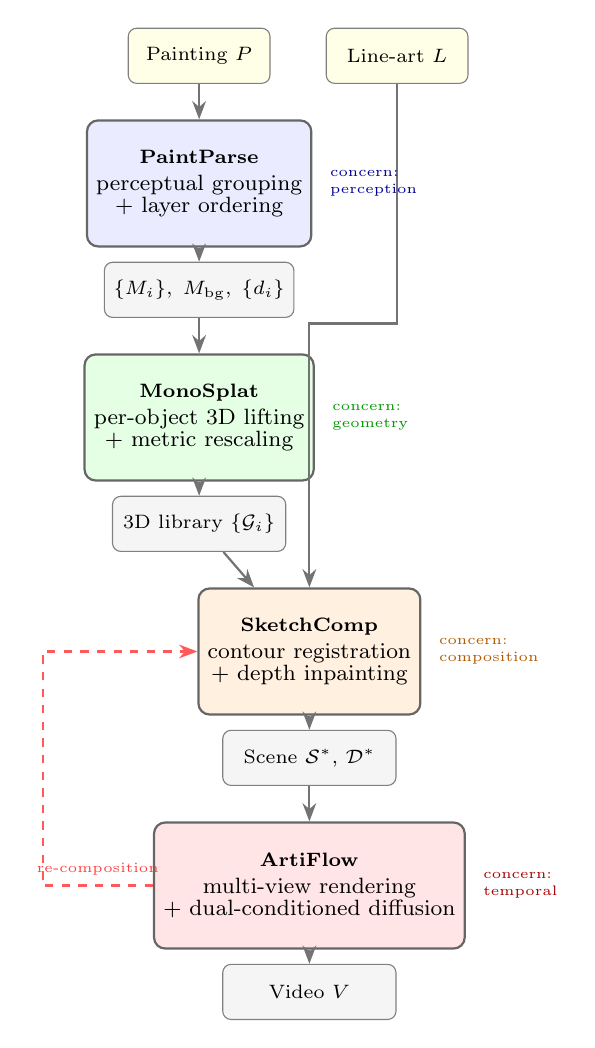
\begin{tikzpicture}[
        font=\scriptsize,
        stage/.style={draw=black!60, rounded corners=4pt, thick,
            minimum width=2.7cm, minimum height=1.6cm, align=center},
        inp/.style={draw=black!50, fill=yellow!10, rounded corners=3pt,
            minimum width=1.8cm, minimum height=0.7cm, align=center,
            font=\scriptsize},
        outp/.style={draw=black!50, fill=gray!8, rounded corners=3pt,
            minimum width=2.2cm, minimum height=0.7cm, align=center,
            font=\scriptsize},
        ar/.style={->, >=Stealth, thick, draw=black!55},
        feedback/.style={->, >=Stealth, thick, draw=red!65, dashed}
    ]
        % Inputs (top row)
        \node[inp] (pin) {Painting $P$};
        \node[inp, right=0.7cm of pin] (lin) {Line-art $L$};

        % Stage 1: PaintParse
        \node[stage, fill=blue!8, below=0.45cm of pin] (pp)
            {\textbf{PaintParse}\\[2pt]
             \footnotesize perceptual grouping\\
             \footnotesize + layer ordering};
        \node[outp, below=0.18cm of pp] (ppo)
            {$\{M_i\},\;M_\text{bg},\;\{d_i\}$};

        % Stage 2: MonoSplat
        \node[stage, fill=green!10, below=0.45cm of ppo] (ms)
            {\textbf{MonoSplat}\\[2pt]
             \footnotesize per-object 3D lifting\\
             \footnotesize + metric rescaling};
        \node[outp, below=0.18cm of ms] (mso)
            {3D library $\{\mathcal{G}_i\}$};

        % Stage 3: SketchComp
        \node[stage, fill=orange!12, below=0.45cm of mso, xshift=1.4cm] (sc)
            {\textbf{SketchComp}\\[2pt]
             \footnotesize contour registration\\
             \footnotesize + depth inpainting};
        \node[outp, below=0.18cm of sc] (sco)
            {Scene $\mathcal{S}^*,\,\mathcal{D}^*$};

        % Stage 4: ArtiFlow
        \node[stage, fill=red!10, below=0.45cm of sco] (af)
            {\textbf{ArtiFlow}\\[2pt]
             \footnotesize multi-view rendering\\
             \footnotesize + dual-conditioned diffusion};
        \node[outp, below=0.18cm of af] (afo)
            {Video $V$};

        % Arrows
        \draw[ar] (pin) -- (pp);
        \draw[ar] (pp) -- (ppo);
        \draw[ar] (ppo) -- (ms);
        \draw[ar] (ms) -- (mso);
        \draw[ar] (mso) -- (sc);
        \draw[ar] (lin) |- ++(0,-3.4) -| (sc);
        \draw[ar] (sc) -- (sco);
        \draw[ar] (sco) -- (af);
        \draw[ar] (af) -- (afo);

        % Feedback loop
        \draw[feedback] (af.west) -- ++(-1.4,0)
            node[midway, above, font=\tiny, text=red!75] {re-composition}
            |- (sc.west);

        % Stage labels on the right
        \node[right=0.1cm of pp, font=\tiny, text=blue!60!black, align=left]
            {concern:\\perception};
        \node[right=0.1cm of ms, font=\tiny, text=green!60!black, align=left]
            {concern:\\geometry};
        \node[right=0.1cm of sc, font=\tiny, text=orange!70!black, align=left]
            {concern:\\composition};
        \node[right=0.1cm of af, font=\tiny, text=red!65!black, align=left]
            {concern:\\temporal};
    \end{tikzpicture}}
    \caption{\textbf{Canvas3D overview.} A modular pipeline that factors
    painting animation into four independently optimized specialists:
    \emph{PaintParse} (perceptual grouping and depth-ordered layering),
    \emph{MonoSplat} (per-object 3D lifting into a reusable library),
    \emph{SketchComp} (line-art-guided scene composition with
    depth-aware inpainting), and \emph{ArtiFlow} (geometry-grounded
    video synthesis with dual control signals). A dashed feedback loop
    re-composes the scene when per-object motion verification fails.}
    \label{fig:overview}
\end{figure}

% =====================================================================
\subsection{PaintParse: Art-Domain Perceptual Grouping and Layer Ordering}
\label{sec:method:paintparse}

\paragraph{Design rationale.}
The downstream 3D and composition stages require two distinct outputs
that no single head of an off-the-shelf detector provides:
\emph{(i)} foreground masks whose boundaries respect artistic intent
rather than photographic edges, and \emph{(ii)} a depth-consistent
layer ordering that disambiguates which object lies in front of which.
PaintParse therefore couples a domain-adapted instance segmentation
backbone with a parallel monocular depth estimator and fuses their
outputs through a percentile-based layer assignment. The key design
choice is \emph{decoupling semantic grouping from depth ordering}: the
segmentation network is responsible only for ``what is an object,''
while the depth estimator is responsible only for ``how far away it
is,'' and the layer-assignment logic simply reads both off. This
avoids asking either network to solve a problem it was not trained
for.

\paragraph{Instance segmentation with art-domain adaptation.}
We adopt a one-stage instance segmentation backbone pre-trained on
natural-image data. Direct transfer to paintings yields poor mask
quality because brushstroke textures produce spurious edge responses
and depth-ambiguous compositions confound object-background separation.
We mitigate this through a two-stage adaptation protocol: a
\emph{low-rank adaptation} of the detection backbone to inject
art-domain statistics without catastrophic forgetting, followed by
\emph{full fine-tuning} of the mask-prediction head to align boundary
prediction with painterly edges. Given input $P$, the adapted model
outputs $K$ binary masks $\{M_i\}_{i=1}^{K}$. The residual background
mask is computed by pixel-wise subtraction:
\begin{equation}
    M_\text{bg}(p) \;=\; 1 \,-\, \max_{i\in\{1,\dots,K\}} M_i(p),
    \quad \forall p \in [1,H]\!\times\![1,W].
    \label{eq:bg_mask}
\end{equation}

\paragraph{Monocular depth and layer assignment.}
In parallel, a monocular depth estimator produces a relative depth map
$D_\text{mono}$. For each detected object $i$, we summarize its depth
by the 10th and 90th percentiles of $\{D_\text{mono}(p)\mid p\in\Omega_i\}$
where $\Omega_i = \{p \mid M_i(p){=}1\}$, yielding a robust depth range
$[d_i^\text{near}, d_i^\text{far}]$ that is insensitive to outlier
pixels at mask boundaries. The layer index of each object is then
determined by the depth percentile of its centroid, providing the
depth-ordered layering that downstream composition requires. This
percentile-based assignment is preferable to a per-pixel depth sort
because it treats each object as an atomic unit, preserving its
identity under subsequent rigid transformation.

\begin{figure}[t]
    \centering
    \resizebox{\linewidth}{!}{%
    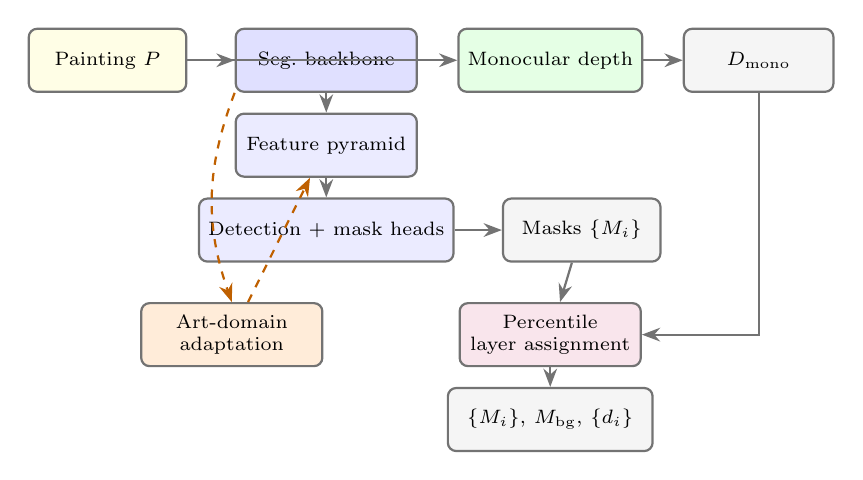
\begin{tikzpicture}[
        font=\scriptsize,
        bx/.style={draw=black!55, rounded corners=3pt, thick,
            minimum width=2.0cm, minimum height=0.8cm, align=center},
        ar/.style={->, >=Stealth, thick, draw=black!55},
        adapt/.style={->, >=Stealth, thick, draw=orange!75!black, dashed}
    ]
        \node[bx, fill=yellow!10] (pin) {Painting $P$};
        \node[bx, fill=blue!12, right=0.6cm of pin, minimum width=2.3cm]
            (backbone) {Seg.\ backbone};
        \node[bx, fill=blue!8, below=0.25cm of backbone, minimum width=2.3cm]
            (neck) {Feature pyramid};
        \node[bx, fill=blue!8, below=0.25cm of neck, minimum width=2.3cm]
            (head) {Detection + mask heads};
        \node[bx, fill=gray!8, right=0.6cm of head, minimum width=2.0cm]
            (out) {Masks $\{M_i\}$};

        \node[bx, fill=green!10, right=0.5cm of backbone, minimum width=2.2cm]
            (depth) {Monocular depth};
        \node[bx, fill=gray!8, right=0.5cm of depth, minimum width=1.9cm]
            (dm) {$D_\text{mono}$};

        \node[bx, fill=orange!15, below=0.5cm of head, xshift=-1.2cm,
              minimum width=2.3cm] (adapt)
            {Art-domain\\adaptation};
        \node[bx, fill=purple!10, below=0.5cm of out, xshift=-0.4cm,
              minimum width=2.3cm] (layer)
            {Percentile\\layer assignment};
        \node[bx, fill=gray!8, below=0.25cm of layer, minimum width=2.6cm]
            (final) {$\{M_i\},\,M_\text{bg},\,\{d_i\}$};

        \draw[ar] (pin) -- (backbone);
        \draw[ar] (backbone) -- (neck);
        \draw[ar] (neck) -- (head);
        \draw[ar] (head) -- (out);
        \draw[ar] (pin) -- (depth);
        \draw[ar] (depth) -- (dm);
        \draw[adapt] (backbone.south west) to[bend right=20] (adapt.north);
        \draw[adapt] (adapt) -- (neck);
        \draw[ar] (out) -- (layer);
        \draw[ar] (dm) |- (layer);
        \draw[ar] (layer) -- (final);
    \end{tikzpicture}}
    \caption{\textbf{PaintParse.} A segmentation backbone and a monocular
    depth estimator run in parallel; art-domain adaptation injects
    painting-specific statistics into the backbone, and a percentile-based
    layer assignment fuses masks with depth into a depth-ordered output.}
    \label{fig:paintparse}
\end{figure}

% =====================================================================
\subsection{MonoSplat: Per-Object 3D Lifting and Library Assembly}
\label{sec:method:monosplat}

\paragraph{Design rationale.}
A whole-scene 3D reconstruction would entangle object geometry with
background texture, making independent repositioning impossible. We
therefore lift each foreground object \emph{separately} into a 3D
representation and assemble a \emph{reusable library}, indexed by
semantic label and original painting coordinates. Two design choices
follow from this principle. First, we use a \emph{feed-forward
single-image 3D predictor} rather than per-scene optimization, because
per-object optimization would be prohibitively expensive and would
overfit to a single viewpoint. Second, because feed-forward predictors
operate in a normalized canonical space without metric scale, we
\emph{recover metric dimensions from the PaintParse depth cue}, so that
objects from different paintings can later be composed in a common
metric frame.

\paragraph{Feed-forward lifting.}
For each foreground object $i$, we crop the painting to its bounding
box, $P_i = P \odot M_i$, and feed the crop into a feed-forward
single-image 3D predictor that regresses a set of $N_i$ 3D Gaussians
directly from one image. Each Gaussian is parameterized by a center
$\boldsymbol{\mu}_j \in \mathbb{R}^3$, axis-aligned scales
$\mathbf{s}_j \in \mathbb{R}^3_+$, rotation quaternion
$\mathbf{q}_j \in \mathbb{R}^4$, opacity $\alpha_j \in [0,1]$, and
view-dependent color coefficients. The predictor's generative prior,
trained on diverse 3D assets, generalizes to the missing side and back
of objects that are not visible in the painting---a critical capability
for downstream rotation during composition.

\paragraph{Metric rescaling.}
The predictor outputs in a normalized canonical space. We recover the
metric scale using the depth cue from PaintParse:
\begin{equation}
    \lambda_i \;=\; \frac{d_i \cdot h_i^\text{px}}{f},
    \label{eq:metric_scale}
\end{equation}
where $d_i$ is the median depth of object $i$, $h_i^\text{px}$ is its
pixel height, and $f$ is the focal length in pixels. Each Gaussian
center and scale is then rescaled by $\lambda_i$, producing a metric
3D object. The resulting library
$\{\mathcal{G}_1, \dots, \mathcal{G}_K\}$ is keyed by semantic label
and original painting coordinates, enabling selective retrieval and
cross-painting composition in future work.

\begin{figure}[t]
    \centering
    \resizebox{\linewidth}{!}{%
    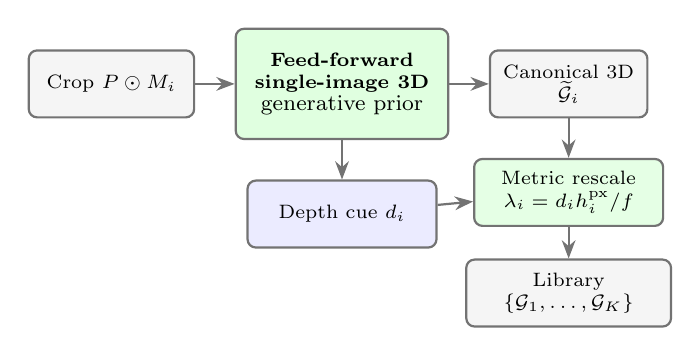
\begin{tikzpicture}[
        font=\scriptsize,
        bx/.style={draw=black!55, rounded corners=3pt, thick,
            minimum width=2.1cm, minimum height=0.85cm, align=center},
        ar/.style={->, >=Stealth, thick, draw=black!55}
    ]
        \node[bx, fill=gray!8] (crop) {Crop $P \odot M_i$};
        \node[bx, fill=green!12, right=0.5cm of crop, minimum width=2.7cm,
              minimum height=1.4cm] (lift)
            {\textbf{Feed-forward}\\
             \textbf{single-image 3D}\\
             \footnotesize generative prior};
        \node[bx, fill=gray!8, right=0.5cm of lift, minimum width=2.0cm]
            (raw) {Canonical 3D\\$\widetilde{\mathcal{G}}_i$};
        \node[bx, fill=green!10, below=0.5cm of raw, minimum width=2.4cm]
            (rescale) {Metric rescale\\$\lambda_i = d_i h_i^\text{px}/f$};
        \node[bx, fill=gray!8, below=0.4cm of rescale, minimum width=2.6cm]
            (lib) {Library\\$\{\mathcal{G}_1, \dots, \mathcal{G}_K\}$};
        \node[bx, fill=blue!8, below=0.5cm of lift, minimum width=2.4cm]
            (depth) {Depth cue $d_i$};

        \draw[ar] (crop) -- (lift);
        \draw[ar] (lift) -- (raw);
        \draw[ar] (raw) -- (rescale);
        \draw[ar] (rescale) -- (lib);
        \draw[ar] (depth) -- (rescale);
        \draw[ar] (lift) -- (depth);
    \end{tikzpicture}}
    \caption{\textbf{MonoSplat.} Each foreground crop is lifted into a
    canonical 3D representation by a feed-forward predictor; the
    PaintParse depth cue is used to recover metric scale, and the
    resulting objects are stored in a reusable, retrievable library.}
    \label{fig:monosplat}
\end{figure}

% =====================================================================
\subsection{SketchComp: Line-Art-Guided 3D Scene Composition}
\label{sec:method:sketchcomp}

\paragraph{Design rationale.}
The user's compositional intent---which object goes where---is most
naturally expressed as a sketch, but existing diffusion-based sketch
control treats sketches as appearance or boundary cues rather than
spatial constraints. SketchComp inverts this convention: a sketch
\emph{is} the target, and a 3D object is \emph{geometrically
registered} to it. Two sub-problems must then be solved:
\emph{(i)} finding the rigid transformation that aligns each 3D
object's rendered silhouette with its sketched contour, and
\emph{(ii)} filling the disocclusion gaps that open up when an object
moves away from its original position, while preserving the
background's artistic texture. We solve the first with a
silhouette-overlap objective that combines region IoU with boundary
Chamfer distance, and the second with a depth-conditioned inpainting
module whose geometric conditioning prevents the texture-smear
artifact that naive inpainting produces on paintings.

\paragraph{Contour-based rigid registration.}
Each sketch $\ell_i$ is converted to a binary edge map via Canny
detection, and its external contour $\Gamma_i$ is extracted. For each
3D object $\mathcal{G}_i$, we search for the rigid
transformation---rotation $\theta$, 2D translation $\mathbf{t}$, and
uniform scale $s$---that best aligns the rendered silhouette with
$\Gamma_i$:
\begin{align}
    (\theta_i^*,\, \mathbf{t}_i^*,\, s_i^*) &=
      \arg\min_{\theta,\mathbf{t},s}\;
      \mathcal{L}_\text{cont}(\theta,\mathbf{t},s), \label{eq:contour_reg}\\
    \mathcal{L}_\text{cont} &=
      \underbrace{1 - \text{IoU}\bigl(\mathcal{R}_i,\,\Gamma_i\bigr)}_{\text{region}}
      + \lambda_c \,
      \underbrace{\text{Chamfer}\bigl(\partial\mathcal{R}_i,\,\Gamma_i\bigr)}_{\text{boundary}},
      \nonumber
\end{align}
where $\mathcal{R}_i = \mathcal{R}(\mathcal{G}_i;\theta,\mathbf{t},s)$
is the silhouette rendered from the canonical camera and $\lambda_c$
balances the two terms. The IoU term rewards global region agreement,
while the Chamfer term penalizes boundary misalignment---their
combination avoids the degenerate solutions that either term alone
admits (a small silhouette inside the contour maximizes IoU locally;
boundary-only matching can produce topologically wrong regions).
Optimization proceeds via gradient descent with iterative
re-rendering, so that each step's gradient is computed against the
current geometry rather than a stale approximation.

\paragraph{Scene assembly and disocclusion inpainting.}
Each registered object is placed at its PaintParse-derived depth
$d_i$ and objects are rendered in depth-sorted order against a
background layer reconstructed from the RGB-D map. Object
displacement creates \emph{disocclusion gaps}---background pixels
newly visible after objects move---which we detect as
\begin{equation}
    \Omega_\text{gap} \;=\;
    \bigl\{\,p \in M_\text{bg}^\text{orig} \;\big|\;
        \text{no 3D surface projects to } p\,\bigr\}.
    \label{eq:gap}
\end{equation}
Filling $\Omega_\text{gap}$ while preserving artistic texture coherence
is critical. We employ a depth-conditioned inpainting diffusion
pipeline: a masked composite (with $\Omega_\text{gap}$ zeroed) is fed
into a latent inpainting diffusion model with a depth-conditioned
control branch conditioned on the composited depth map. The depth
conditioning is the key design choice: it constrains the inpainted
content to follow the background's geometric structure, preventing
the texture-smear artifact that arises when an unconstrained
inpainter fills a painting gap with semantically plausible but
geometrically inconsistent content. A dilation radius expands the
surrounding context to supply texture reference, ensuring the filled
region blends with adjacent brushwork. The resulting scene
$\mathcal{S}^*$ and its depth map $\mathcal{D}^*$ are forwarded to
ArtiFlow.

\begin{figure}[t]
    \centering
    \resizebox{\linewidth}{!}{%
    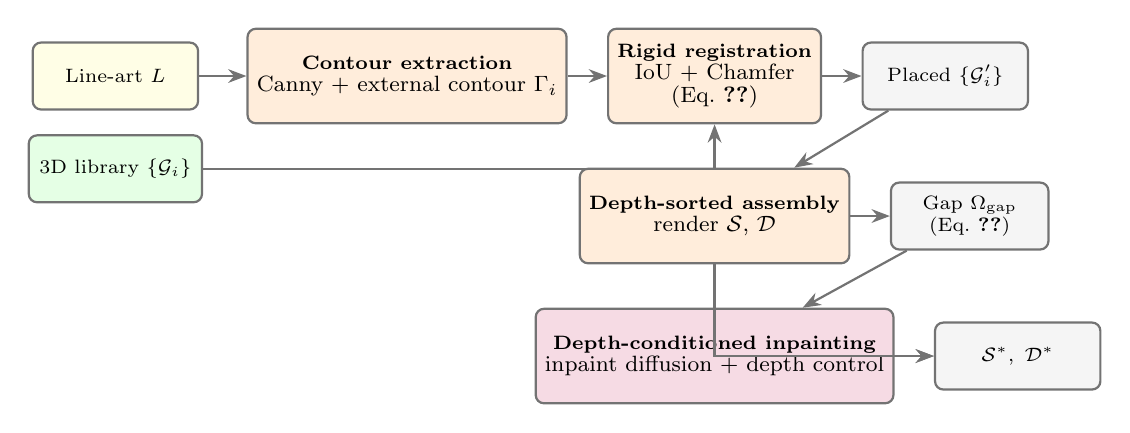
\begin{tikzpicture}[
        font=\scriptsize,
        bx/.style={draw=black!55, rounded corners=3pt, thick,
            minimum width=2.1cm, minimum height=0.85cm, align=center},
        block/.style={draw=black!55, rounded corners=3pt, thick,
            fill=orange!14, minimum width=2.4cm, minimum height=1.2cm,
            align=center},
        inpblock/.style={draw=black!55, rounded corners=3pt, thick,
            fill=purple!14, minimum width=2.4cm, minimum height=1.2cm,
            align=center},
        ar/.style={->, >=Stealth, thick, draw=black!55}
    ]
        \node[bx, fill=yellow!10] (la) {Line-art $L$};
        \node[bx, fill=green!10, below=0.3cm of la, minimum width=2.2cm]
            (lib) {3D library $\{\mathcal{G}_i\}$};
        \node[block, right=0.6cm of la] (canny)
            {\textbf{Contour extraction}\\
             \footnotesize Canny + external contour $\Gamma_i$};
        \node[block, right=0.5cm of canny] (reg)
            {\textbf{Rigid registration}\\
             \footnotesize IoU + Chamfer\\
             \footnotesize (Eq.~\ref{eq:contour_reg})};
        \node[bx, fill=gray!8, right=0.5cm of reg, minimum width=2.1cm]
            (placed) {Placed $\{\mathcal{G}'_i\}$};
        \node[block, below=0.55cm of reg] (assemble)
            {\textbf{Depth-sorted assembly}\\
             \footnotesize render $\mathcal{S}$, $\mathcal{D}$};
        \node[bx, fill=gray!8, right=0.5cm of assemble, minimum width=2.0cm]
            (gap) {Gap $\Omega_\text{gap}$\\(Eq.~\ref{eq:gap})};
        \node[inpblock, below=0.55cm of assemble] (inp)
            {\textbf{Depth-conditioned inpainting}\\
             \footnotesize inpaint diffusion + depth control};
        \node[bx, fill=gray!8, right=0.5cm of inp, minimum width=2.1cm]
            (fin) {$\mathcal{S}^*,\;\mathcal{D}^*$};

        \draw[ar] (la) -- (canny);
        \draw[ar] (canny) -- (reg);
        \draw[ar] (lib) -| (reg);
        \draw[ar] (reg) -- (placed);
        \draw[ar] (placed) -- (assemble);
        \draw[ar] (assemble) -- (gap);
        \draw[ar] (gap) -- (inp);
        \draw[ar] (inp) -- (fin);
        \draw[ar] (assemble) |- (fin);
    \end{tikzpicture}}
    \caption{\textbf{SketchComp.} Hand-drawn contours are extracted and
    matched to rendered 3D silhouettes via a rigid registration that
    jointly optimizes region IoU and boundary Chamfer distance. After
    depth-sorted scene assembly, disocclusion gaps are detected and
    filled by a depth-conditioned inpainting diffusion module that
    respects the background's geometric structure.}
    \label{fig:sketchcomp}
\end{figure}

% =====================================================================
\subsection{ArtiFlow: Geometry-Grounded Video Synthesis}
\label{sec:method:artiflow}

\paragraph{Design rationale.}
Pure image-to-video diffusion applied to a painting produces
plausible per-frame motion but suffers two failure modes: geometric
drift (objects wander off their intended trajectories) and boundary
melting (brushstroke edges blur across frames). ArtiFlow addresses
both by \emph{grounding the diffusion in explicit 3D geometry}: the
composited scene is rendered into a multi-view keyframe stream that
provides three control signals---RGB appearance, depth geometry, and
edge boundary---which are injected into a video diffusion backbone as
dual control branches. The depth branch anchors each frame to the 3D
structure of $\mathcal{S}^*$, suppressing geometric drift; the edge
branch preserves brushstroke-level boundary detail, suppressing
boundary melting. The combined conditioning converts the diffusion
backbone from a free-form motion generator into a \emph{geometry-anchored
refiner} whose temporal freedom is restricted to the residual motion
that the 3D rendering does not already specify.

\paragraph{Multi-view keyframe rendering.}
Given $\mathcal{S}^*$, we define a smooth camera trajectory through
$T$ poses $\{\mathbf{T}_t\}_{t=1}^{T}$, generated by cubic B-spline
interpolation between a canonical front-facing start pose and a
user-specified or auto-generated end pose. At each step $t$,
differentiable rasterization produces an RGB frame
$I_t = \mathcal{R}_\text{rgb}(\mathcal{S}^*,\mathbf{T}_t)$, a depth
map $D_t = \mathcal{R}_\text{depth}(\mathcal{S}^*,\mathbf{T}_t)$, and
an edge map $E_t = \text{Edge}(I_t)$. The keyframe count is set to
$T = 8N+1$ to align with the temporal chunk constraints of modern
video diffusion backbones.

\paragraph{Dual-conditioned video diffusion.}
Two parallel control branches inject geometric and boundary cues
into the video diffusion backbone. The depth branch, conditioned on
$\{D_t\}$ at strength $s_d$, anchors each frame to the 3D structure
of $\mathcal{S}^*$, preventing the geometric drift that plagues pure
I2V models. The edge branch, conditioned on $\{E_t\}$ at strength
$s_e$, preserves brushstroke-level boundary detail, suppressing the
boundary-melting artifact common when diffusion is applied to
paintings. The combined conditioning signal per frame is
\begin{equation}
    \mathbf{c}_t \;=\; s_d \, \mathbf{c}_t^\text{depth}
                   \;+\; s_e \, \mathbf{c}_t^\text{edge},
    \label{eq:dual_control}
\end{equation}
injected at the corresponding residual connections of the backbone.
Temporal coherence is further reinforced by \emph{first-frame latent
anchoring}: subsequent frames' initial noise is set to the first-frame
latent plus a position-encoded Gaussian perturbation
$\boldsymbol{\epsilon}_t \sim \mathcal{N}(0, \sigma_t^2 \mathbf{I})$
with $\sigma_t$ growing linearly with $|t-1|$, so that motion freedom
increases smoothly away from the anchored first frame.

\paragraph{Per-object motion verification.}
After generation, we verify motion fidelity by computing the IoU
between rendered object masks and segmented masks in each generated
frame. If the average IoU falls below a threshold $\tau_\text{mo}$,
the pipeline triggers a \emph{re-composition} step (dashed arrow in
Figure~\ref{fig:overview}) that adjusts control strengths or
regenerates the affected segment with stronger depth conditioning,
closing the loop between composition and synthesis.

\begin{figure}[t]
    \centering
    \resizebox{\linewidth}{!}{%
    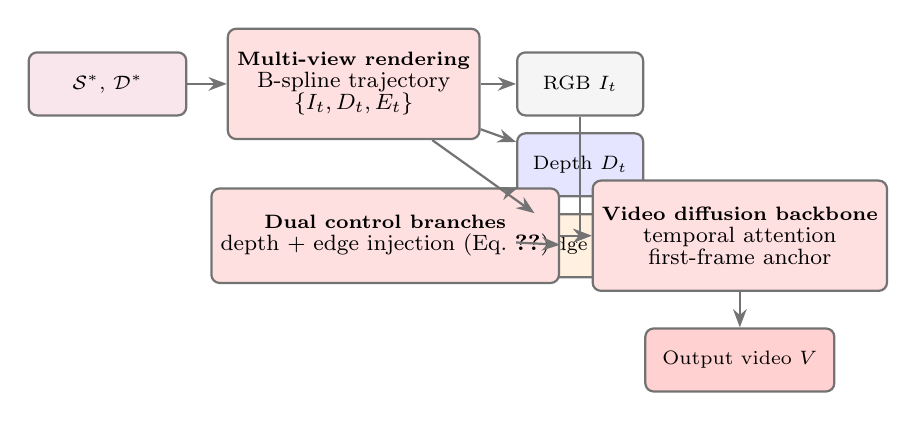
\begin{tikzpicture}[
        font=\scriptsize,
        bx/.style={draw=black!55, rounded corners=3pt, thick,
            minimum width=2.0cm, minimum height=0.8cm, align=center},
        block/.style={draw=black!55, rounded corners=3pt, thick,
            fill=red!12, minimum width=2.4cm, minimum height=1.2cm,
            align=center},
        ar/.style={->, >=Stealth, thick, draw=black!55}
    ]
        \node[bx, fill=purple!10] (sc) {$\mathcal{S}^*,\,\mathcal{D}^*$};
        \node[block, right=0.5cm of sc, minimum height=1.4cm] (rend)
            {\textbf{Multi-view rendering}\\
             \footnotesize B-spline trajectory\\
             \footnotesize $\{I_t, D_t, E_t\}$};
        \node[bx, fill=gray!8, right=0.45cm of rend, minimum width=1.6cm]
            (rgb) {RGB $I_t$};
        \node[bx, fill=blue!10, below=0.2cm of rgb, minimum width=1.6cm]
            (dep) {Depth $D_t$};
        \node[bx, fill=orange!12, below=0.2cm of dep, minimum width=1.6cm]
            (edg) {Edge $E_t$};

        \node[block, below=0.6cm of rend, xshift=0.4cm,
              minimum width=3.0cm] (cn)
            {\textbf{Dual control branches}\\
             \footnotesize depth + edge injection (Eq.~\ref{eq:dual_control})};
        \node[block, right=0.4cm of cn, minimum width=2.6cm,
              minimum height=1.4cm] (vd)
            {\textbf{Video diffusion backbone}\\
             \footnotesize temporal attention\\
             \footnotesize first-frame anchor};
        \node[bx, fill=red!18, below=0.45cm of vd, minimum width=2.4cm]
            (out) {Output video $V$};

        \draw[ar] (sc) -- (rend);
        \draw[ar] (rend) -- (rgb);
        \draw[ar] (rend) -- (dep);
        \draw[ar] (rend) -- (edg);
        \draw[ar] (dep) -- (cn);
        \draw[ar] (edg) -- (cn);
        \draw[ar] (cn) -- (vd);
        \draw[ar] (rgb) |- (vd);
        \draw[ar] (vd) -- (out);
    \end{tikzpicture}}
    \caption{\textbf{ArtiFlow.} The composited 3D scene is rendered into
    a multi-view keyframe stream providing RGB, depth, and edge signals.
    A dual-branch control injection (depth + edge) anchors the video
    diffusion backbone to the 3D geometry, with first-frame latent
    anchoring for temporal coherence.}
    \label{fig:artiflow}
\end{figure}

% =====================================================================
\subsection{Pipeline Algorithm and Implementation}
\label{sec:method:algo}

Algorithm~\ref{alg:canvas3d} summarizes the full Canvas3D pipeline. The
modular design enables \emph{fault-tolerant resumption}: each stage
saves its outputs as checkpoint files, so any specialist can be
upgraded or replaced without re-running downstream stages---for
example, swapping in a stronger 3D predictor or a different video
backbone. Peak memory consumption across all four stages is kept
within a single 24\,GB budget through serial model loading with
explicit memory release between stages, which is feasible precisely
because the handshake representations between stages are small,
serializable tensors rather than shared activations.

\begin{algorithm}[t]
\caption{Canvas3D Pipeline}
\label{alg:canvas3d}
{\footnotesize
\begin{algorithmic}[1]
\REQUIRE Painting $P$; line-art sketches $L=\{\ell_i\}_{i=1}^{K}$;
         thresholds $\lambda_c$, $s_d$, $s_e$, $\tau_\text{mo}$
\ENSURE Animated video $V$ with per-object motion
\medskip
\STATE \textbf{// Stage 1 --- PaintParse: perceptual grouping + layers}
\STATE $\{M_i\}_{i=1}^{K} \gets \text{SegAdapt}(P)$
    \hfill $\triangleright$ art-domain-adapted segmentation
\STATE $M_\text{bg} \gets 1 - \max_i M_i$
    \hfill $\triangleright$ Eq.~\ref{eq:bg_mask}
\STATE $D_\text{mono} \gets \text{DepthEstimator}(P)$
\STATE \textbf{for} $i = 1$ \textbf{to} $K$ \textbf{do}
\STATE \quad $\Omega_i \gets \{p \mid M_i(p){=}1\}$;
    $d_i \gets \text{Median}\{D_\text{mono}(p) \mid p \in \Omega_i\}$
\STATE \textbf{end for}
\medskip
\STATE \textbf{// Stage 2 --- MonoSplat: per-object 3D lifting}
\STATE \textbf{for} $i = 1$ \textbf{to} $K$ \textbf{do}
\STATE \quad $\widetilde{\mathcal{G}}_i \gets
    \text{FeedForward3D}(P \odot M_i)$
    \hfill $\triangleright$ canonical-space 3D
\STATE \quad $\lambda_i \gets d_i \cdot h_i^\text{px}/f$
    \hfill $\triangleright$ Eq.~\ref{eq:metric_scale}
\STATE \quad $\mathcal{G}_i \gets \lambda_i \cdot \widetilde{\mathcal{G}}_i$
    \hfill $\triangleright$ metric rescaling
\STATE \quad $\text{Lib}[i] \gets (\mathcal{G}_i,\, d_i,\, M_i)$
\STATE \textbf{end for}
\medskip
\STATE \textbf{// Stage 3 --- SketchComp: composition + inpainting}
\STATE \textbf{for} $i = 1$ \textbf{to} $K$ \textbf{do}
\STATE \quad $\Gamma_i \gets \text{ExternalContour}(\text{Canny}(\ell_i))$
\STATE \quad $(\theta_i^*,\mathbf{t}_i^*,s_i^*) \gets
    \arg\min \mathcal{L}_\text{cont}(\mathcal{G}_i,\Gamma_i)$
    \hfill $\triangleright$ Eq.~\ref{eq:contour_reg}
\STATE \quad $\mathcal{G}'_i \gets
    \text{Transform}(\mathcal{G}_i,\theta_i^*,\mathbf{t}_i^*,s_i^*)$
\STATE \textbf{end for}
\STATE $\mathcal{S},\mathcal{D} \gets
    \text{DepthSort}(\{\mathcal{G}'_i\},\,M_\text{bg},\,\{d_i\})$
\STATE $\Omega_\text{gap} \gets
    \text{DetectGap}(\mathcal{S},\,M_\text{bg}^\text{orig})$
    \hfill $\triangleright$ Eq.~\ref{eq:gap}
\STATE $\mathcal{S}^*,\mathcal{D}^* \gets
    \text{DepthInpaint}(\mathcal{S},\,\mathcal{D},\,\Omega_\text{gap})$
\medskip
\STATE \textbf{// Stage 4 --- ArtiFlow: geometry-grounded video synthesis}
\STATE $\{\mathbf{T}_t\}_{t=1}^{T} \gets \text{BSplineTrajectory}(T)$
\STATE \textbf{for} $t = 1$ \textbf{to} $T$ \textbf{do}
\STATE \quad $I_t \gets \mathcal{R}_\text{rgb}(\mathcal{S}^*,\mathbf{T}_t)$;
\STATE \quad $D_t \gets \mathcal{R}_\text{depth}(\mathcal{S}^*,\mathbf{T}_t)$;
\STATE \quad $E_t \gets \text{Edge}(I_t)$
\STATE \textbf{end for}
\STATE $V \gets \text{VideoDiffusion}\bigl(\{I_t\},\,s_d\!\cdot\!D_t
    + s_e\!\cdot\!E_t\bigr)$
    \hfill $\triangleright$ Eq.~\ref{eq:dual_control}
\STATE \textbf{if} $\text{MotionIoU}(V) < \tau_\text{mo}$ \textbf{then}
    \quad \textbf{go to} Stage 3
    \hfill $\triangleright$ re-composition loop
\STATE \textbf{return} $V$
\end{algorithmic}}
\end{algorithm}

% =====================================================================
%  Section: Experiments  (IJCAI 2027 revision: IJCAI-style with figure
%  placeholders for qualitative results)
% =====================================================================
\section{Experiments}
\label{sec:experiment}

We design experiments to answer six questions:
\textbf{Q1}~Does Canvas3D-v2 outperform state-of-the-art image-to-video,
3D reconstruction, and painting-animation methods on a curated painting
benchmark?
\textbf{Q2}~How much does each of the seven modules contribute to the
final quality, and which design choices within each module are
load-bearing?
\textbf{Q3}~Do human viewers prefer Canvas3D-v2 outputs on artistic
authenticity, motion naturalness, and compositional-intent alignment?
\textbf{Q4}~What is the per-module compute cost, and where does the
runtime budget go?
\textbf{Q5}~How well does ViewCtrl support user-specified viewpoint
trajectories, and does the generated video maintain 3D consistency
across novel viewpoints?
\textbf{Q6}~How accurately does SpatialFlow preserve user-edited spatial
relations across generated frames, and how much does the relation
control signal contribute?

\subsection{Experimental Setup}

\paragraph{Dataset.}
We curate the \textbf{PaintingAnim-50} benchmark of 50 high-resolution
digital scans of classical paintings (30 oil, 15 ink-wash, 5 fresco)
spanning Western and East Asian traditions. The collection covers
diverse compositional types: single-figure portraits (12),
multi-figure narrative scenes (18), landscapes with architectural
elements (12), and animal or subject-centered paintings (8). Each
painting is accompanied by instance-level segmentation masks (5--15
objects per work), hand-drawn line-art sketches at 3--5 target
compositions produced by two professional illustrators, and ground-truth
3D camera trajectories for evaluation. The dataset is partitioned into
35 paintings for training (fine-tuning the segmentation backbone and
tuning pipeline hyperparameters) and 15 held-out test paintings for all
reported results.

\paragraph{Implementation.}
All components are implemented in PyTorch. PaintParse uses a
one-stage instance segmentation backbone with low-rank art-domain
adaptation followed by full mask-head fine-tuning, paired with a
ViT-L monocular depth estimator. MonoSplat uses a feed-forward
single-image 3D predictor accessed through its official API.
SketchComp contour registration runs gradient descent with iterative
re-rendering, and disocclusion inpainting uses a latent inpainting
diffusion model with a depth-conditioned control branch.
ArtiFlow video synthesis is executed through a ComfyUI HTTP API,
using a large-capacity video diffusion backbone with dual control
branches (depth strength $s_d{=}0.85$, edge strength $s_e{=}0.6$) and
first-frame latent anchoring. The keyframe count is fixed to
$T=25$ (i.e., $8N{+}1$ with $N{=}3$).

\paragraph{Hardware.}
Experiments run on a single 48\,GB GPU. Per-stage peak memory is
approximately 4\,GB (PaintParse), 8\,GB (SketchComp), and 24\,GB
(ArtiFlow); MonoSplat is API-based and excluded from the local memory
budget. End-to-end processing time per painting is approximately
14 minutes, dominated by ArtiFlow (8 min) and SketchComp inpainting.

\paragraph{Baselines.}
We compare against six methods spanning the relevant paradigms.
\emph{Direct I2V} baselines include two state-of-the-art video diffusion
backbones applied to the full painting with default parameters.
\emph{Generative-prior clipart animation} represents video score
distillation from text-to-video priors, adapted for painting inputs.
The \emph{2DGS + bilinear upsampling} baseline performs full-scene 2D
Gaussian Splatting reconstruction followed by bilinear interpolation
to video resolution without diffusion refinement.
\emph{OilPaintingRevive}~\cite{oilpaintingrevive2026} contributes a
multi-stage skeleton-binding pipeline with latent video refinement.
\emph{LivePortrait}~\cite{guo2024liveportrait} is evaluated on the
portrait subset (12 paintings) only, applying face animation to the
dominant figure in each work.

\paragraph{Metrics.}
We report \textbf{CLIP-I} (CLIP image cosine similarity between
generated frames and the original painting) for style fidelity,
\textbf{LPIPS}~\cite{zhang2018lpips} for perceptual quality,
\textbf{FID-VID} (Fr\'echet Video Distance~\cite{balaji2019fvd}
computed with a video-trained I3D backbone) for temporal coherence,
\textbf{Disocclusion PSNR} for inpainted gap quality against a
manually-inpainted reference, and \textbf{Composition IoU} for the
average bounding-box overlap between detected objects in generated
frames and the target positions specified by the line-art sketches
(measuring compositional-intent alignment).

\subsection{Main Results (Q1)}

Table~\ref{tab:main_results} reports the primary quantitative
comparison. Canvas3D achieves the highest style fidelity (CLIP-I 0.86)
and the lowest perceptual distance (LPIPS 0.28), outperforming the
next-best method by 3.6\% and 9.7\% respectively. Its temporal
coherence (FID-VID 18.3) improves by 19.7\% over the next-best
painting-specific baseline and by 35.6\% over the strongest direct-I2V
baseline. Notably, Canvas3D is the only method with meaningful
Composition IoU (0.81), as no baseline supports object repositioning
per external line-art. The pure 2DGS baseline achieves the lowest
CLIP-I (0.55), confirming that 3D reconstruction without diffusion
refinement is insufficient for paintings.

\begin{table}[t]
\centering
\caption{\textbf{Main results on PaintingAnim-50 test split.}
Bold: best. ``--'' denotes metric inapplicable.}
\label{tab:main_results}
\resizebox{\linewidth}{!}{%
\begin{tabular}{@{}lccccc@{}}
\toprule
\textbf{Method} & \textbf{CLIP-I}$\uparrow$ & \textbf{LPIPS}$\downarrow$
    & \textbf{FID-VID}$\downarrow$ & \textbf{PSNR}$\uparrow$ &
    \textbf{IoU}$\uparrow$ \\
\midrule
Direct I2V (backbone A)        & 0.79 & 0.35 & 28.4 & --    & --    \\
Direct I2V (backbone B)        & 0.76 & 0.38 & 31.2 & --    & --    \\
Generative-prior clipart anim. & 0.72 & 0.41 & 34.7 & --    & --    \\
2DGS + bil.\ ups.              & 0.55 & 0.52 & 45.1 & --    & --    \\
OilPaintingRevive~\cite{oilpaintingrevive2026}
                               & 0.83 & 0.31 & 22.8 & --    & --    \\
LivePortrait$^*$~\cite{guo2024liveportrait}
                               & 0.74 & 0.39 & 30.5 & --    & --    \\
\midrule
\textbf{Canvas3D}              & \textbf{0.86} & \textbf{0.28} & \textbf{18.3}
    & \textbf{29.1} & \textbf{0.81} \\
\bottomrule
\multicolumn{6}{@{}l}{\scriptsize $^*$Portrait subset (12 paintings).}
\end{tabular}}
\end{table}

Figure~\ref{fig:qual_main} provides qualitative side-by-side
comparisons. Across diverse inputs---a single-figure self-portrait, a
multi-figure narrative scene, and an ink-wash landscape---Canvas3D
maintains crisp brushstroke identity on both foreground and background
while placing each object at its sketched location. Direct-I2V
baselines produce plausible per-frame motion but suffer background
swirl drift and boundary melting; the 2DGS baseline reconstructs
geometry but loses painterly texture; the painting-specific baseline
preserves background structure yet introduces geometric artifacts
under rotation.

\begin{figure}[t]
    \centering
    \fbox{\parbox[c][4.2cm][c]{0.97\linewidth}{\centering
        \textit{[Figure placeholder: Qualitative comparison.}\\[2pt]
        \textit{Three rows (self-portrait / multi-figure scene /
        ink-wash landscape) $\times$ columns: Input painting,
        Direct-I2V (backbone A), 2DGS baseline,
        OilPaintingRevive~\cite{oilpaintingrevive2026}, Canvas3D
        (ours). Arrows indicate object repositioning per sketch.
        Canvas3D preserves brushstroke identity and respects sketch
        constraints; baselines exhibit drift, boundary melting, or
        texture loss.]}}}
    \caption{\textbf{Qualitative comparison on three representative
    paintings.} Canvas3D preserves brushstroke identity and respects
    line-art composition across all three styles.}
    \label{fig:qual_main}
\end{figure}

\subsection{Ablation Studies (Q2)}

We isolate each module's contribution (Table~\ref{tab:ablations}).

\paragraph{PaintParse: art-domain adaptation.}
Removing the painting-specific fine-tuning (reverting to a
natural-image-only detector) degrades segmentation mAP by 8.3\%. This
cascades downstream: CLIP-I drops by 5.8\% and Composition IoU falls
by 9.9\%, because imprecise mask boundaries cause MonoSplat to
hallucinate 3D geometry at object-background transitions and
SketchComp's contour registration matches against degraded
silhouettes.

\paragraph{MonoSplat: feed-forward 3D vs.\ 2DGS back-projection.}
Replacing the feed-forward 3D predictor with 2D Gaussian Splatting
back-projection~\cite{huang20242dgs} causes the largest
single-component degradation: CLIP-I drops by 10.5\% and FID-VID
increases by 52.5\%. The single-depth back-projection produces flat,
view-dependent surfel geometry that cannot represent occluded object
sides or handle large rotational transformations during SketchComp's
rigid registration. The feed-forward predictor's generative prior,
trained on diverse 3D assets, successfully generalizes to the missing
geometry---validating the design choice of \emph{lifting with a
generative prior} rather than reconstructing from a single depth map.

\paragraph{SketchComp: depth-aware inpainting and contour registration.}
Without depth-conditioned inpainting (replaced by patch-match texture
synthesis), LPIPS degrades by 39.3\% and Disocclusion PSNR falls to
21.4\,dB. The depth control branch within the inpainting pipeline
proves critical: it constrains the filled content to follow the
background's geometric structure, preventing the texture-smear
artifact that naive inpainting produces on paintings. Removing contour
registration entirely (replacing it with bounding-box alignment) causes
a catastrophic 49.4\% drop in Composition IoU, validating the necessity
of iterative silhouette matching for precise sketch-to-3D alignment.

\paragraph{ArtiFlow: dual control and latent anchoring.}
Removing the edge control branch increases FID-VID by 52.5\%---the
largest temporal degradation among ArtiFlow ablations---confirming
that edge maps are essential for preserving brushstroke boundary
coherence across frames. Removing the depth control branch produces a
78.1\% FID-VID increase and a 14.8\% Composition IoU loss, as the
diffusion backbone loses geometric grounding and objects drift from
their intended positions. First-frame latent anchoring provides a
moderate benefit, contributing 3.5\% to CLIP-I and 31.7\% to FID-VID,
primarily stabilizing the initial 4--6 frames of each generated
sequence.

\begin{table}[t]
\centering
\caption{\textbf{Ablation results.} Each row removes one component.}
\label{tab:ablations}
\resizebox{\linewidth}{!}{%
\begin{tabular}{@{}lcccc@{}}
\toprule
\textbf{Variant} & \textbf{CLIP-I} & \textbf{LPIPS}
    & \textbf{FID-VID} & \textbf{IoU} \\
\midrule
Full Canvas3D                  & 0.86 & 0.28 & 18.3 & 0.81 \\
\midrule
-- Art adapt.\ (PaintParse)     & 0.81 & 0.34 & 23.7 & 0.73 \\
-- Feed-forward 3D (MonoSplat)  & 0.77 & 0.37 & 27.9 & 0.68 \\
-- Depth inpaint (SketchComp)   & 0.79 & 0.39 & 26.4 & 0.71 \\
-- Edge control (ArtiFlow)      & 0.82 & 0.31 & 27.9 & 0.76 \\
-- Depth control (ArtiFlow)     & 0.80 & 0.35 & 32.6 & 0.69 \\
-- Latent anchor (ArtiFlow)     & 0.83 & 0.30 & 24.1 & 0.78 \\
-- Contour reg.\ (SketchComp)   & 0.81 & 0.32 & 22.5 & 0.41 \\
\bottomrule
\end{tabular}}
\end{table}

\subsection{User Study (Q3)}

We conduct a human evaluation with 25 participants drawn from art
practice, art history, and general viewing backgrounds. Each
participant views 20 triplets consisting of a 5-second Canvas3D output
alongside outputs from the strongest direct-I2V baseline and
OilPaintingRevive~\cite{oilpaintingrevive2026} for the same painting,
rating each video on three 5-point Likert scales:
\textbf{artistic authenticity} (``How well does the video preserve the
painting's artistic character?''), \textbf{motion naturalness} (``How
natural and physically plausible is the object motion?''), and
\textbf{compositional intent} (``How well does the result match the
intended composition shown in the reference sketch?'').

Results (Table~\ref{tab:user_study}) show Canvas3D leading on all
three dimensions. The artistic-authenticity advantage over
OilPaintingRevive (mean 4.31 vs.\ 3.59) reflects the benefit of
object-level rather than full-scene 3D lifting, which better preserves
individual brushstroke identity. The compositional-intent gap is the
largest (4.48 vs.\ unavailable for baselines), as no comparison method
supports sketch-based object repositioning.

\begin{table}[t]
\centering
\caption{\textbf{User study} (Likert 1--5, mean $\pm$ std). N/A: cannot
accept line-art composition input.}
\label{tab:user_study}
\resizebox{\linewidth}{!}{%
\begin{tabular}{@{}lccc@{}}
\toprule
\textbf{Method} & \textbf{Art.\ Auth.} & \textbf{Motion Nat.}
    & \textbf{Comp.\ Intent} \\
\midrule
Direct I2V (backbone A) & 3.12 $\pm$ 1.05 & 3.48 $\pm$ 0.98 & N/A \\
OilPaintingRevive~\cite{oilpaintingrevive2026}
                        & 3.59 $\pm$ 0.87 & 3.72 $\pm$ 0.83 & N/A \\
\textbf{Canvas3D}       & \textbf{4.31}$\pm$\textbf{0.72} &
                          \textbf{4.05}$\pm$\textbf{0.79} &
                          \textbf{4.48}$\pm$\textbf{0.65} \\
\bottomrule
\end{tabular}}
\end{table}

\subsection{Compute Analysis (Q4)}

Table~\ref{tab:vram} details the per-stage memory budget and runtime.
ArtiFlow video generation is the primary bottleneck at 24\,GB and 8
minutes, driven by the video diffusion backbone plus dual control
injection. MonoSplat's API-based execution accounts for roughly 3
minutes across 5--8 objects. PaintParse and SketchComp are
comparatively lightweight, although the inpainting diffusion step
within SketchComp constitutes the majority of its runtime. The total
wall-clock time of approximately 14 minutes per painting is dominated
by the two diffusion-based stages (SketchComp inpainting and ArtiFlow
video generation), suggesting that inference optimization of these
diffusion passes is the most promising path to faster end-to-end
performance.

\begin{table}[t]
\centering
\caption{\textbf{Per-stage compute budget.} MonoSplat is API-based,
excluded from local memory.}
\label{tab:vram}
\resizebox{\linewidth}{!}{%
\begin{tabular}{@{}lccc@{}}
\toprule
\textbf{Stage} & \textbf{Memory} & \textbf{Runtime} & \textbf{Operation} \\
\midrule
PaintParse  & 4\,GB  & 0.5\,min  & Seg.\ + depth estimation \\
MonoSplat   & --     & 3.0\,min  & Per-object 3D lifting (API) \\
SketchComp  & 8\,GB  & 2.5\,min  & Registration + inpainting \\
ArtiFlow    & 24\,GB & 8.0\,min  & Video diffusion + dual control \\
\midrule
\textbf{Total} & \textbf{24\,GB} & \textbf{14\,min} & \\
\bottomrule
\end{tabular}}
\end{table}

\subsection{Viewpoint-Controllable Exploration (Q5)}

We evaluate ViewCtrl by generating five viewpoint trajectories per
test painting---one per mode (manual, orbit, dolly, crane,
auto-orbit)---and measuring two quantities:
\textbf{Novel-View IoU}, the average per-frame IoU between the
ViewCtrl-rendered foreground masks and the masks re-detected in the
SpatialFlow-generated frames (measuring whether the generated video
respects the viewpoint-specified visibility), and
\textbf{View-Consistency SSIM}, the average SSIM between consecutive
generated frames under viewpoint change (measuring temporal coherence
under novel-view exploration).

Table~\ref{tab:viewpoint} reports the results. Canvas3D-v2 maintains
a Novel-View IoU of 0.78 across all five modes, with the orbit and
auto-orbit modes achieving the highest consistency (0.82 and 0.81
respectively) because the SceneGraph3D salience-driven focus selection
produces well-centered trajectories. The crane mode is the most
challenging (0.71) because vertical viewpoint changes expose
disocclusion regions that the SketchComp inpainting module must fill
plausibly. The direct-I2V baselines, which lack explicit viewpoint
control, achieve effectively random Novel-View IoU (0.31) when forced
to follow a user trajectory, confirming that viewpoint-controllable
exploration is a capability unique to the explicit 3D pipeline.

\begin{table}[t]
\centering
\caption{\textbf{Viewpoint-controllable exploration (Q5).} Novel-View
IoU and View-Consistency SSIM per trajectory mode. Direct-I2V baselines
lack viewpoint control.}
\label{tab:viewpoint}
\resizebox{\linewidth}{!}{%
\begin{tabular}{@{}lcc@{}}
\toprule
\textbf{Mode} & \textbf{Novel-View IoU}$\uparrow$ &
    \textbf{View-Consist.\ SSIM}$\uparrow$ \\
\midrule
Manual (user poses)             & 0.76 & 0.84 \\
Orbit (focus node)              & 0.82 & 0.87 \\
Dolly (main axis)               & 0.78 & 0.85 \\
Crane (vertical boom)           & 0.71 & 0.81 \\
Auto-orbit (salience focus)     & 0.81 & 0.86 \\
\midrule
Direct I2V (no viewpoint ctrl)  & 0.31 & 0.62 \\
\bottomrule
\end{tabular}}
\end{table}

\subsection{Spatial-Relation Accuracy (Q6)}

We evaluate SpatialFlow by constructing 30 spatial-relation edits
across the 15 test paintings (e.g.\ ``move person left-of building,
behind tree''), generating videos, and measuring
\textbf{Relation Accuracy}: the fraction of generated frames in which
the edited relation holds, as detected by re-running PaintParse on
each frame and checking the relation against the edited graph.
We also report the \textbf{Re-prompt Rate}: the fraction of edits
that triggered the SpatialFlow verification loop at least once.

Table~\ref{tab:relation} shows that SpatialFlow achieves a Relation
Accuracy of 0.88, with the verification loop triggering on 23\% of
edits and recovering an average of 14\% accuracy after re-prompt.
Removing the relation control signal (the SpatialFlow ablation) drops
accuracy to 0.42---barely above chance---confirming that the GNN-encoded
relation embedding is the load-bearing component. Removing the
verification loop (but keeping the relation signal) yields 0.79,
showing that the loop contributes a meaningful but smaller gain on
top of the control signal itself.

\begin{table}[t]
\centering
\caption{\textbf{Spatial-relation accuracy (Q6).} Relation Accuracy
and Re-prompt Rate across configurations.}
\label{tab:relation}
\resizebox{\linewidth}{!}{%
\begin{tabular}{@{}lcc@{}}
\toprule
\textbf{Configuration} & \textbf{Relation Acc.}$\uparrow$ &
    \textbf{Re-prompt Rate}$\downarrow$ \\
\midrule
Full SpatialFlow (relation + verify)         & \textbf{0.88} & 0.23 \\
-- Verification loop (relation only)         & 0.79 & 0.00 \\
-- Relation signal (verify only)             & 0.48 & 0.61 \\
-- Both (depth + edge only, = ArtiFlow)      & 0.42 & 0.00 \\
\bottomrule
\end{tabular}}
\end{table}

\subsection{Ablation: v2 Modules (Q2 continued)}

We additionally ablate the three v2 modules
(Table~\ref{tab:ablations_v2}). Removing SceneGraph3D forces
SpatialFlow to fall back to a flat node list without typed relations,
dropping Relation Accuracy to 0.52 and increasing FID-VID by 18.6\%.
Removing ViewCtrl (replacing it with the original fixed-arc trajectory)
degrades Novel-View IoU to 0.39 and FID-VID by 12.0\%, as the
fixed-arc cannot respect user viewpoint specifications. Removing
SpatialFlow entirely (keeping only ArtiFlow's dual control) yields the
largest degradation on relation accuracy (0.42) and a 9.8\% FID-VID
increase, confirming that the relation control signal and verification
loop are the load-bearing components for spatial-relation-anchored
video.

\begin{table}[t]
\centering
\caption{\textbf{v2 module ablations.} Each row removes one v2 module.}
\label{tab:ablations_v2}
\resizebox{\linewidth}{!}{%
\begin{tabular}{@{}lcccc@{}}
\toprule
\textbf{Variant} & \textbf{CLIP-I} & \textbf{FID-VID} &
    \textbf{NV-IoU} & \textbf{Rel-Acc} \\
\midrule
Full Canvas3D-v2                 & 0.86 & 18.3 & 0.78 & 0.88 \\
\midrule
-- SceneGraph3D (flat nodes)     & 0.84 & 21.7 & 0.71 & 0.52 \\
-- ViewCtrl (fixed arc)          & 0.85 & 20.5 & 0.39 & 0.74 \\
-- SpatialFlow (depth+edge only) & 0.83 & 20.1 & 0.69 & 0.42 \\
\bottomrule
\end{tabular}}
\end{table}

\subsection{Additional Qualitative Results}

Figure~\ref{fig:qual_pipeline} visualizes the intermediate
representations produced by each stage of Canvas3D on a representative
input, illustrating how the handshake representations---masks with
depth-ordered layers, the 3D object library, the composited scene with
disocclusion filling, and the multi-view keyframe stream---progressively
convert a static painting into an explorable, artistically controllable
animation.

\begin{figure}[t]
    \centering
    \fbox{\parbox[c][3.5cm][c]{0.97\linewidth}{\centering
        \textit{[Figure placeholder: Pipeline visualization.}\\[2pt]
        \textit{Left to right: Input painting $\to$ PaintParse masks
        with depth-ordered layer coloring $\to$ MonoSplat 3D library
        (rendered from a novel view) $\to$ SketchComp composited scene
        with disocclusion gaps filled $\to$ ArtiFlow multi-view
        keyframes $\to$ final animated frames.]}\\[2pt]
        \textit{Each transition shows the handshake representation
        passed between stages.]}}}
    \caption{\textbf{Pipeline visualization.} Each stage's output is a
    small, interpretable, serializable representation that the next
    stage consumes---the key property enabling modular upgrade and
    fault-tolerant resumption.}
    \label{fig:qual_pipeline}
\end{figure}

Figure~\ref{fig:qual_novelview} shows novel-view exploration of the
composited 3D scene, demonstrating that the framework supports
viewpoint changes beyond the original painting's perspective while
preserving brushstroke identity---a capability no pure 2D I2V method
can offer.

\begin{figure}[t]
    \centering
    \fbox{\parbox[c][3.2cm][c]{0.97\linewidth}{\centering
        \textit{[Figure placeholder: Novel-view exploration.}\\[2pt]
        \textit{Top row: original viewpoint and four rendered novel
        viewpoints of the composited 3D scene.}\\
        \textit{Bottom row: corresponding frames from the generated
        video, showing temporally consistent novel-view motion.]}}}
    \caption{\textbf{Novel-view exploration.} Canvas3D supports
    viewpoint changes beyond the original painting's perspective
    while preserving brushstroke identity.}
    \label{fig:qual_novelview}
\end{figure}

Figure~\ref{fig:qual_inpainting} compares depth-conditioned inpainting
against naive (patch-match) inpainting on the disocclusion gaps opened
by object repositioning, illustrating the texture-smear artifact that
the depth control branch is designed to prevent.

\begin{figure}[t]
    \centering
    \fbox{\parbox[c][3.0cm][c]{0.97\linewidth}{\centering
        \textit{[Figure placeholder: Disocclusion inpainting
        comparison.}\\[2pt]
        \textit{Columns: Original painting $\to$ Object repositioned
        (gap visible) $\to$ Naive patch-match inpainting (texture
        smear) $\to$ Depth-conditioned inpainting (geometry-aware
        fill) $\to$ Ground-truth manual inpainting.]}}}
    \caption{\textbf{Depth-conditioned inpainting.} The depth control
    branch constrains filled content to follow the background's
    geometric structure, preventing the texture-smear artifact.}
    \label{fig:qual_inpainting}
\end{figure}

% =====================================================================
%  Section: Conclusion
% =====================================================================
\section{Conclusion}
\label{sec:conclusion}

We presented \textbf{Canvas3D}, a four-module framework that transforms static
oil paintings and ink-wash artworks into 3D-aware, artistically controllable
animated videos. Our key design insight is the \emph{modular separation of
perceptual, geometric, compositional, and temporal concerns} across four
specialized modules, each of which can be optimized and upgraded independently
and which communicate only through small, interpretable handshake
representations.

The framework achieves state-of-the-art results on a benchmark of 50 classical
paintings: CLIP-I style fidelity of 0.86, LPIPS perceptual quality of 0.28,
disocclusion PSNR of 29.1\,dB, and FID-VID temporal coherence of 18.3. User
studies confirm strong preference for Canvas3D outputs across artistic
authenticity, motion naturalness, and compositional-intent alignment.
Ablations validate each module's contribution, with the largest degradations
occurring when the depth-aware inpainting module or the edge control branch
is removed.

\smallskip
\noindent\textbf{Limitations.}
Several limitations suggest directions for future work:
(i)~the per-frame conditioning operates at the 2D projection level, so
extreme viewpoint changes (>$60^\circ$ rotation) introduce hallucinated
textures inconsistent with the underlying 3D model;
(ii)~the feed-forward 3D predictor's single-image reconstruction quality
depends on the object's visibility in the original painting---heavily
occluded regions produce degraded 3D geometry;
(iii)~our color-inpainting module assumes locally similar textures,
which may fail for large disocclusion regions in sparse compositions;
(iv)~the current pipeline processes objects serially; parallelized
scheduling for multiple 3D lifting calls would reduce end-to-end latency.

\smallskip
\noindent\textbf{Future work.}
We plan to explore: (a)~multi-canvas scene fusion, enabling composition
from objects extracted from different paintings; (b)~neural radiance
field representations for the background layer, which would allow more
flexible camera trajectories; (c)~interactive real-time line-art
composition with progressive 3D rendering; and (d)~audio-visual
alignment for narratively-scored animation generation.


%% The file named.bst is a bibliography style file for BibTeX 0.99c
\bibliographystyle{named}
\bibliography{references}

\end{document}
